% !TEX root = ./main.tex
\section{Results}
\subsection{Genes studied}
\tr{Does this belong into results or introduction?}
In total we present the regulatory architecture of x promoters, which tells us how a total of y genes are regulated. 18 promoters were chosen as so called "gold standards". These genes have well annotated promoters and have been studied in detail in previous experiments \cite{belliveau2018systematic,ireland2020deciphering}. Including this set of genes allows us to compare the method presented in this work to previous iterations and verify the results, as well as find possible derivations or improvements. x promoters were chosen for genes that have been identified to have a high variation in protein copy number \tr{Probably should show that in the SI} across a set of 22 growth conditions by Schmidt et al., 2016 \cite{schmidt2016quantitative}. These genes were chosen since a high variation in copy number suggests that there are regulatory proteins controlling the expression of the gene. From the same dataset, a set of x promoters was chosen for genes with unidentified function, as annotated by the Schmidt et al., 2016 \cite{schmidt2016quantitative}. None of these promoters had any regulatory annotation prior to the experiments. Another set of x promoters were chosen for genes that were identified in EcoCyc as not having any functional annotation. Two groups of genes, so called iModulons \cite{lamoureux2021precise} were chosen from the work of Lamoureux et al. 2021, where ca. 800 RNA-Seq datasets were evaluated to find genes that were regulated in a distinct network. \tr{Give details for iModulons and their function in their respective paragraphs?} The \tr{Give summary of all genes at the end of this paragragh.}
\tr{Continue with genes of defined circuits and toxin/antitoxin genes}

\subsection{Genome Integration of Reporters}
A major improvement to the Reg-Seq method is the genome integration of the reporter using ORBIT (see supplementary information \ref{sec:genome_int}). By integrating the mutated promoter into the genome instead of keeping it on a plasmid, the variation in copy number per cell is reduced and the total number of reporters per cell is at an absolute minimum. Transcription factors that bind to the native version of the promoter in the chromosome also bind to the promoter copy, unless its binding site is heavily mutated. Hence, if many promoter copies are added to a cell, e.g. via plasmids, transcription factors are more likely to bind the promoter of the reporter \cite{brewster2014transcription}, leading to possible fitness defects of the cell. During the cloning process the reporters are carried on a plasmid with a copy number on the order of 10 (r6k replication origin). This effect can be seen in the results of the barcode mapping for the promoter of the gene \textit{dicC}. In the promoter there is a binding site for DicA between the -9 and +11 positions (relative to the transcription start site), which was not identifiable in the previous iteration of Reg-Seq \cite{ireland2020deciphering}. The sequences obtained for this promoter on our barcode mapping show an increased mutation rate in exactly the site predicted to be the transcription factor binding site, see Supplementary Figure \ref{fig:dicCp}. This means that sequences without mutations in this part of the promoter were not able to be cloned and lead to fitness defects, presumably due to the transcription factor being titrated away from the native promoter in the chromosome.

\subsection{Barcode Mapping}

\subsection{Transcription Factor identification}
\subsection{Growth Conditions}
\begin{figure}
    \centering
    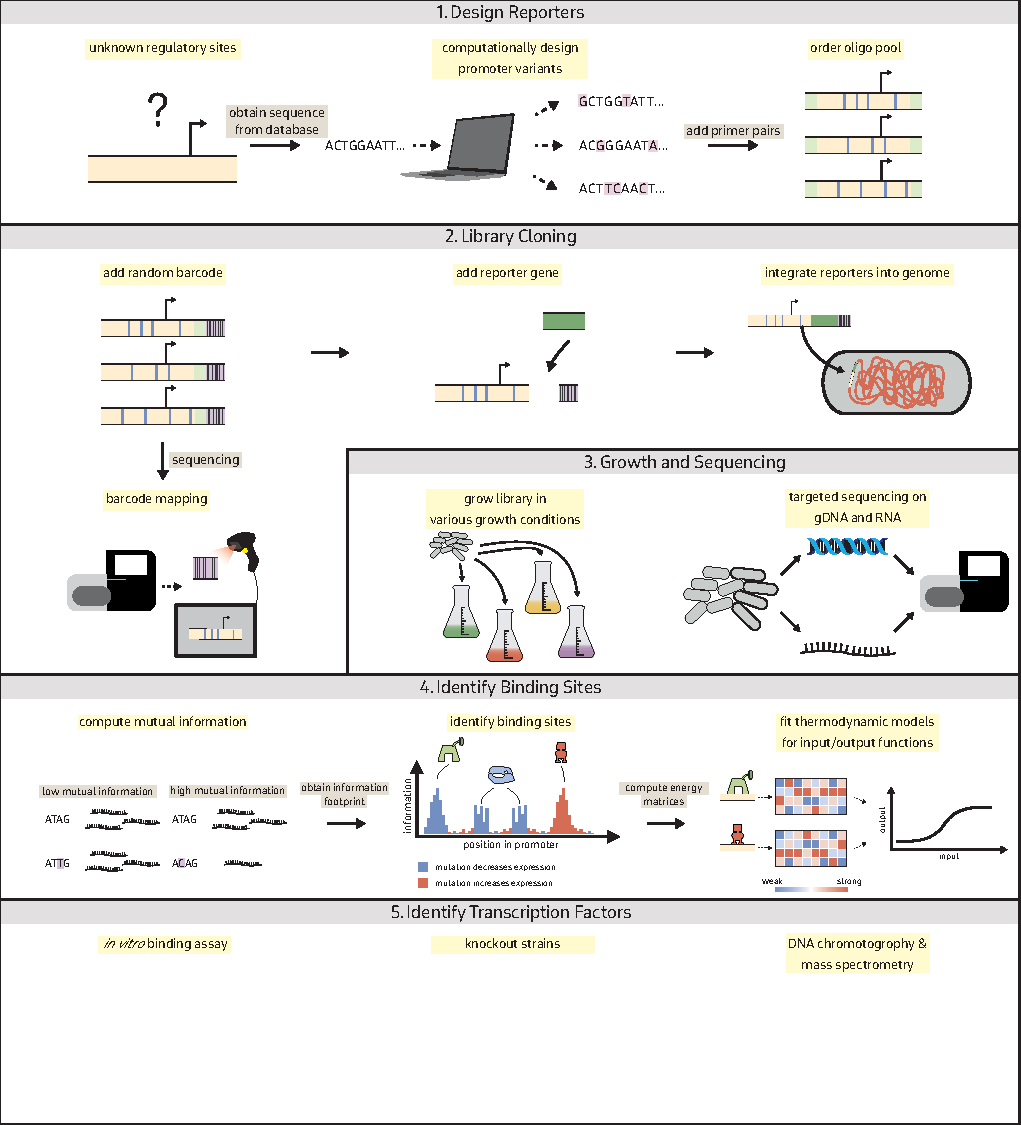
\includegraphics{../figures/figure2_method_sum.pdf}
    \caption{Method summary}
    \label{fig:method_sum}
\end{figure}
\subsection{Gold Standard genes}
\subsection{Ethanol iModulon}
YgeV has been predicted to be a regulator involved in purine catabolism, leading to the production of allantoin, which can be used as a sole nitrogen source \cite{iwadate2019identification}. There are 16 putative regulatory targets \cite{lamoureux2021precise} for YgeV, including the \textit{xdhABC} operon, which degrades xanthine to uric acid \cite{iwadate2019identification} in the purine catabolism pathway. \textit{E. coli} can survive exposure to low ethanol concentrations up to 5\%, which can even lead to increased DNA synthesis \cite{basu1994effect}, but mostly leads to varies stress responses such as an increased production of ROS. Growth in media supplemented with ethanol induced a change in gene expression for genes regulated by YgeV in a \textDelta\textit{baeR} or \textDelta\textit{cpxR} mutant strain. \tr{Is there a correlation between ethanol response and higher need for nitrogen?}
\subsection{Oxidative stress response iModulon}
The putative transcription factor YmfT regulates 14 out of 23 genes in the e14 prophage and is predicted to respond to oxidative stress \cite{lamoureux2021precise}. Oxidative stress is caused by reactive oxygen species (ROS) such as $\text{H}_2\text{O}_2$, which are highly reactive and damage DNA, the cell wall, proteins \cite{ezraty2017oxidative} etc., however, oxidized amino acids can also lead to confirmational changes in transcription factors, such as OxyR and HypT, which induce DNA binding and subsequent regulation of genes involved in response to oxidative stress  \cite{ezraty2017oxidative}. Hydrogen peroxide is produced endogenously in various pathways in \textit{E. coli} and especially in high amounts when phenylethylamine is used as either carbon or nitrogen source \cite{ravindra2013escherichia}, hence we used used minimal media supplemented with 10 mM 2-phenylethylamine hydrochloride (PEA) as sole carbon source to induce stress responses to $\text{H}_2\text{O}_2$ and therefore oxidative stress. \tr{discuss findings of ymfT modulon and how it relates to oxyR, look at oxyR iModulons and possibly do another run including this gene.}
\subsection{Antitoxin/Antibiotic genes}
\subsection{other y-ome genes}
